%%%%%%%%%%%%%%%%%%%%%%%%%%%%%%%%%%%%%%%%%
% Medium Length Graduate Curriculum Vitae
% LaTeX Template
% Version 1.1 (9/12/12)
%
% This template has been downloaded from:
% http://www.LaTeXTemplates.com
%
% Original author:
% Rensselaer Polytechnic Institute (http://www.rpi.edu/dept/arc/training/latex/resumes/)
%
% Modified By:
% Oscar Neiva
% oscar-neiva.github.io 
% oscarneivaeneto@gmail.com
%
% Important note:
% This template requires the res.cls file to be in the same directory as the
% .tex file. The res.cls file provides the resume style used for structuring the
% document.
%
%%%%%%%%%%%%%%%%%%%%%%%%%%%%%%%%%%%%%%%%%

%----------------------------------------------------------------------------------------
%	PACKAGES AND OTHER DOCUMENT CONFIGURATIONS
%----------------------------------------------------------------------------------------

\documentclass[margin, 10pt]{res} % Use the res.cls style, the font size can be changed to 11pt or 12pt here
\usepackage{graphics}
\usepackage{epsfig}
\usepackage{helvet} % Default font is the helvetica postscript font
\usepackage[utf8]{inputenc}
%\usepackage{newcent} % To change the default font to the new century schoolbook postscript font uncomment this line and comment the one above
%\usepackage[lmargin=2.5cm,rmargin=2cm,tmargin=2cm,bmargin=2cm]{geometry}
\setlength{\textwidth}{5.1in} % Text width of the document

\begin{document}

%----------------------------------------------------------------------------------------
%	NAME AND ADDRESS SECTION
%----------------------------------------------------------------------------------------
\moveleft\hoffset\vbox{\hrule width\resumewidth height 1pt}\smallskip %

\vspace{-0.2cm}
\hspace{-3.0cm}
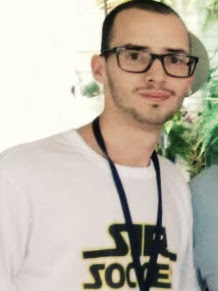
\includegraphics[width=2.2cm]{figures/profile.jpg}

\vspace{-3cm}
\leftline{\large\bf Oscar Neiva} % Your name at the top
\vspace{0.5cm}
\leftline{oscarneivaeneto@gmail.com}
\leftline{oscar-neiva.github.io}
\leftline{Rio de Janeiro, RJ}
 
\vspace{0.8cm}

\moveleft\hoffset\vbox{\hrule width\resumewidth height 1pt}\smallskip % Horizontal line after name; adjust line thickness by changing the '1pt'
 


%----------------------------------------------------------------------------------------

\begin{resume}

%----------------------------------------------------------------------------------------
%	Objetivo e Interesse
%----------------------------------------------------------------------------------------
 
%\section{Objetivo e Interesse}  
%Estagiar na área de desenvolvimento de software.

%----------------------------------------------------------------------------------------
%	Experiência
%----------------------------------------------------------------------------------------
 
\section{Experiência}
{\sl Iniciação Científica} \hfill Maio de 2014 - Março de 2016\\
Laboratório Nacional de Computação Científica - LNCC, Petrópolis, RJ 
\begin{itemize} \itemsep -2pt % Reduce space between items
\item Meu trabalho no LNCC teve como motivação o estudo e simulação de sistemas sujeitos a saltos markovianos, com o objetivo de ao final do trabalho ser feita uma simulação do algoritmo PageRank, o algoritmo por trás da ferramenta de busca do Google.
\end{itemize}

{\sl Estágio em Desenvolvimento de Software} \hfill Abril de 2014 - Dezembro de 2015\\
Laboratório de Sistemas Inteligentes e Robótica - SIRLab, Petrópolis, RJ 
\begin{itemize} \itemsep -2pt % Reduce space between items
\item Trabalhei no SIRLab como desenvolvedor de software em linguagem C++. O projeto do qual fiz parte consistiu em desenvolver um sistema autônomo de futebol de robôs para a categoria IEEE Very Small Size Soccer. Dentre as diversas partes que constituiram o desenvolvimento do sistema SIRSoccer, fui encarregado de pesquisar um modelo de controle adequado e de criar um algoritmo com tal modelo.
\end{itemize}

%----------------------------------------------------------------------------------------
%	Formação Acadêmica
%----------------------------------------------------------------------------------------

\section{Formação Acadêmica}
Faculdade de Educação Tecnológica do Estado do Rio de Janeiro - FAETERJ \\
{\sl Tecnólogo,} Tecnologia da Informação e Comunicação, Petrópolis, RJ, 2013 - 2016.

Colégio M3 \\
Segundo Grau, Niterói, RJ, 2009 - 2011.
 
%----------------------------------------------------------------------------------------
%	Idiomas
%----------------------------------------------------------------------------------------

\section{Idiomas}
{\sl Português,} Nativo.\\
{\sl Inglês,} Avançado.

%----------------------------------------------------------------------------------------
%	Competências
%----------------------------------------------------------------------------------------

\section{Competências} 
{\sl Linguagens \& Softwares:} C, C++, Linux, OpenGL, OpenCV, Arduino, Matlab, Octave, LaTeX, HTML, CSS, Microsoft Excel.

{\sl Outras:} Teoria de Sistema e Controle, Controle de sistemas em tempo real, engrenagens de busca, processos estocásticos.
 
%----------------------------------------------------------------------------------------
%	Cursos e Atividades Extracurriculares
%----------------------------------------------------------------------------------------

\section{Cursos e Atividades Extracurriculares} 
X Escola Luso-Brasileira de Computação Evolutiva, LNCC, fevereiro de 2014.\\
IX Escola de Verão do Laboratório Associado de Computação e Matemática Aplicada, INPE, fevereiro de 2015.\\
Processos de Lévy Aplicados a Finança, LNCC, janeiro de 2015.\\

%----------------------------------------------------------------------------------------
%	Prêmios
%----------------------------------------------------------------------------------------

\section{Prêmios} 
RUNNER-UP in category RoboCup Simulation 2D, LARC/CBR, October 23, 2014.\\
Destaque na Jornada de Iniciação Científica e Tecnológica, LNCC, Setembro, 2015.


%----------------------------------------------------------------------------------------
%	Trabalho Voluntário
%---------------------------------------------------------------------------------------- 

\section{Trabalho Voluntário}
Árbitro na Olimpíada Brasileira de Robótica (estadual Rio de Janeiro), agosto 2014.\\
Organizador da Olimpíada Brasileira de Robótica (regional Petrópolis), agosto 2015.

%----------------------------------------------------------------------------------------

\end{resume}
\end{document}